\documentclass[11pt,oneside]{book}
\usepackage[margin=1in]{geometry}
\usepackage[toc,page]{appendix}
\usepackage{graphicx}
\usepackage{natbib}
\usepackage{lipsum}
\usepackage{caption}
\usepackage{graphicx}

 
\usepackage[bottom]{footmisc}

% disable chapter default name
\usepackage{titlesec}
\titleformat{\chapter}{\normalfont\huge}{\thechapter.}{20pt}{\huge}


% change the title of the table of contents
\renewcommand{\contentsname}{Indice}

% change the title of the list of images
\renewcommand{\listfigurename}{Indice de imagens}

% paragraph spacing
\usepackage{indentfirst}
\setlength{\parindent}{3em}

% for links
\usepackage{hyperref}


\begin{document}

\captionsetup[figure]{margin=1.5cm,font=small,labelfont={bf},name={Figure},labelsep=colon,textfont={it}}
\captionsetup[table]{margin=1.5cm,font=small,labelfont={bf},name={Table},labelsep=colon,textfont={it}}
\setlipsumdefault{1}

\frontmatter

\begin{titlepage}


% -------------------------------------------------------------------
% You need to edit the details here
% -------------------------------------------------------------------

\begin{center}
{\LARGE Universidade de Aveiro}\\[7cm]
\linespread{1.2}\huge {\bfseries HW1: Mid-term assignment report }\\[0.5cm]
\linespread{1}
% \includegraphics[width=7.5cm]{images/soc.png}\\[1cm]
{\large{Pedro Miguel Nicolau Escaleira \textit{[88821]} }}\\
{\large{\url{https://github.com/oEscal/tqs_project_1}}}\\
\vspace*{\fill}
\large{15 de abril, 2020}
\end{center}

\end{titlepage}


% -------------------------------------------------------------------
% Contents
% -------------------------------------------------------------------

\tableofcontents

\listoffigures



% -------------------------------------------------------------------
% Main sections (as required)
% -------------------------------------------------------------------

\mainmatter

% !TEX root = ../main.tex

\chapter{Introdução}

\section{Contextualização do trabalho}
Este projeto, proposto pelo professor da disciplina de \textbf{Teste e Qualidade de Software}, teve como
principal objetivo a consolidação dos conhecimentos adquiridos durante as aulas da mesma tidas até ao momento.

Desta forma, foi sugerida a criação duma aplicação \textit{web} simples para obtenção de dados sobre a 
qualidade do ar num dado sitio fornecido. Para isso, a solução criada possui um \textit{back-end} sob a forma de 
\textit{REST API}, feita em \textit{java} com a ajuda de \textit{Spring Boot} e um \textit{fron-end} feito em 
\textit{python} com a ajuda de \textit{Flask} e \textit{Jinja 2}. Fazendo jus ao nome da disciplina, claramente
toda esta plataforma foi criada com o intuito de serem feitos testes, a vários níveis, para a mesma, pelo que foi,
duma forma geral, usado o \textit{JUnit} para a criação de testes para a \textit{api} e \textit{Selenium WebDriver}
para a criação de testes para a interface.

\section{Limitações}
Apesar do trabalho ter sido concluído com sucesso e de ter ido de encontro aos requisitos pedidos, 
houveram algumas \textit{features} que ficaram por implementar, mas que teriam sido uma adição que o autor
gostaria de ter criado. De seguida, são apresentadas as principais:

\begin{itemize}
   \item \textbf{Pesquisa dum lugar pelo nome}: no resultado final, apenas dá para pesquisar a qualidade de 
ar quando dadas as coordenadas da localização pretendida. Contudo, seria mais \textit{user friendly} fazer a mesma
pesquisa por nome.
   \item \textbf{Utilização doutra \textit{API} remota}: na solução final, apenas é usada um serviço remoto para
obtenção dos dados necessários. Contudo, tal como é sugerido nos pontos extra do guião do trabalho, seria mais
\textit{reliable} a utilização de mais que um serviço, para o caso do primeiro falhar. Esta aproximação não foi usada
já que iria adicionar uma grande quantidade de sobrecarga sobre o trabalho feito dada a dificuldade desta adição 
quando concluído grande parte do código feito.
   \item \textbf{Testes da interface em que houvesse alteração do código \textit{HTML}}: Seria algo de interesse de se
fazer testes, por exemplo, sob \textit{inputs} com atributos alterados, para testar o comportamento da plataforma
quando não apresentada, por exemplo, uma entrada na forma de número ou a submissão do formulário sem quaisquer 
\textit{inputs} obrigatórios preenchidos. Contudo, após alguma pesquisa, o \textit{Selenium IDE}, ferramenta usada
na criação dos testes da interface, não parece apresentar documentação de como fazer alterações no código fonte da
página testada.
\end{itemize}

% !TEX root = ../main.tex

\chapter{Especificações do produto}

\section{Funcionalidades e interações suportadas}
Como demonstrado na figura \ref{fig:interface_current}, esta plataforma é uma aplicação simples que permite aos seus 
utilizadores obterem a qualidade do ar para um determinado lugar, indicando as coordenadas. Permite não só
saber a qualidade atual, mas também a passada e futura. As métricas que ela disponibiliza são a \textbf{data 
referente à qualidade do ar}, o \textbf{valor escalar e textual da qualidade do ar}, o \textbf{poluente 
dominante} e a \textbf{concentração e valor escalar e textual da qualidade do ar referente a cada um dos
poluentes principais}.

\begin{figure}[h]
   \centering
   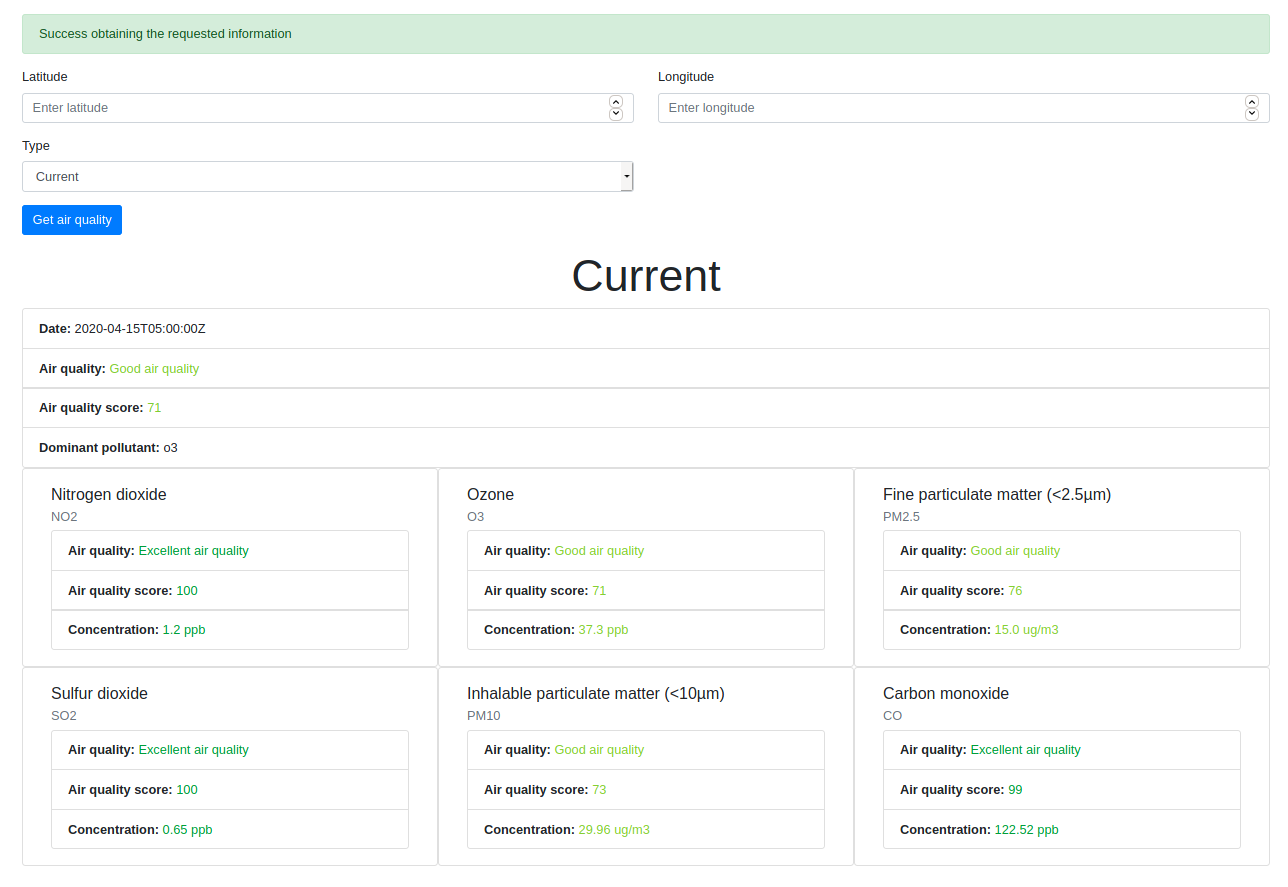
\includegraphics[width=0.90\textwidth]{images/interface_current}
   \caption{\textit{Print} da interface quando feito um pedido da qualidade do ar atual.}
   \label{fig:interface_current}
\end{figure}

Os possíveis utilizadores e cenários da plataforma criada são:

\begin{itemize}
   \item \textbf{População de risco}: dado o estado debilitado desta fração de população, é do interesse 
de algumas saber a qualidade do ar que respiram, principalmente as que possuem problemas respiratórios, 
de forma a melhor controlarem o seu estado de saúde. Desta forma, uma pessoa nestas condições poderá dirigir-se
à interface desta aplicação, introduzir as coordenadas do local onde se encontra ou se vai encontrar nos próximos
tempos, selecionar a obtenção de dados sobre o estado atual (\textit{Type Current}) ou sobre o estado previsto no 
futuro (\textit{Type Forecast}, selecionando também o número de horas seguintes sobre as quais pretende obter os 
dados) e, sendo assim, obter o estado da qualidade do ar atual ou nas horas seguintes, respetivamente.
   \item \textbf{Estudiosos}: profissionais que tenham interesse em estudar a qualidade de ar de acordo com 
o local, como por exemplo o estudo da evolução num determinado lugar. Sendo assim, um utilizador deste tipo
pode dirigir-se à página \textit{web}, selecionar um determinado lugar introduzindo as correspondentes coordenadas,
se pretende os dados de previsões passadas (\textit{Type History}) ou futuras (\textit{Type Forecast}) e o 
número de horas de dados deste o momento atual pretende obter. A partir dos resultados obtidos, poderá copiar
cada um deles e fazer o correspondente estudo.
\end{itemize}


\section{Arquitetura do sistema}
O \textit{back-end} do projeto foi feito usando \textit{java} com \textit{Maven} e \textit{Spring Boot}.
Quanto á arquitetura, é apresentado um diagrama de classes simples da mesma na figura 
\ref{fig:simple_diagram} (este diagrama de classes apenas contém as classes criadas e as relações entre elas,
sendo que os detalhes de cada uma se encontrarão definidos em diagramas expostos em subsecções seguintes, 
de forma a que este não fique demasiado confuso). Estas classes foram organizadas, de acordo com 
a sua complexidade em 4 \textit{packages}: \textbf{controller}, \textbf{model}, \textbf{serializers} e 
\textbf{service}. Nas subsecções seguintes

\begin{figure}[h]
   \centering
   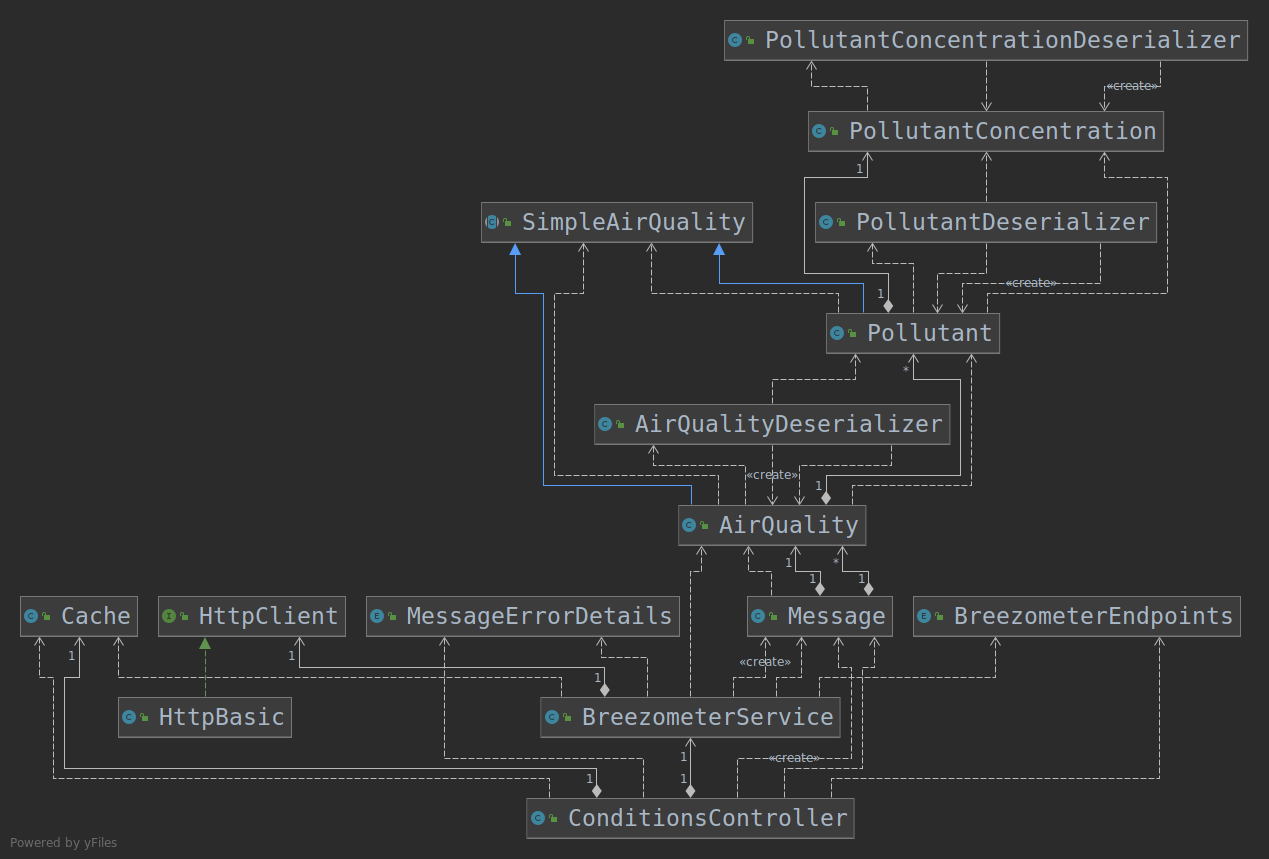
\includegraphics[width=0.90\textwidth]{images/simple_diagram}
   \caption{Diagrama de classes simples do projeto.}
   \label{fig:simple_diagram}
\end{figure}


\subsection{Package controller}
Este \textit{package} é constituído apenas por uma classe, \textbf{\textit{ConditionsController}}, que é
a responsável por lidar com as ligações feitas à \textit{API} criada. Desta forma, nesta classes são
definidos os \textit{endpoints} do nosso serviço e é definida a forma como cada \textit{request} vai ser
consumido no \textit{back-end}. Na figura \ref{fig:controller_diagram} é possível encontrar o esquema da
classe descrita.

\begin{figure}[h]
   \centering
   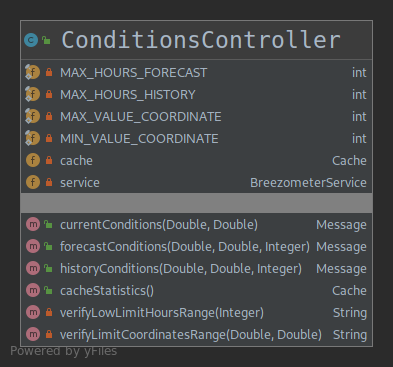
\includegraphics[width=0.40\textwidth]{images/controller_diagram}
   \caption{Diagrama das classes do \textit{package \textbf{controller}}.}
   \label{fig:controller_diagram}
\end{figure}


\subsection{Package model}
Todas as entidades usadas pelo nosso servido são representadas pelas classes deste \textit{package}. Desta forma, nela estão incluídas as classes:
\begin{itemize}
   \item \textbf{Que representam os dados da qualidade do ar}: 
      \begin{itemize}
         \item \textbf{\textit{AirQuality}}: representa a qualidade do ar referente a um determinado momento. Sendo assim, para além dos objetos desta classe possuírem informações básicas sobre a qualidade do ar, contêm também uma lista de poluentes (classe \textbf{\textit{Pollutant}}) que se encontram no ar no instante que esse objeto retrata.
         \item \textbf{\textit{Pollutant}}: classe que contém informações sobre um determinado poluente, como a forma como o respetivo poluente afeta a qualidade do ar e a concentração deste num determinado momento (classe \textbf{\textit{PollutantConcentration}}).
         \item \textbf{\textit{PollutantConcentration}}: classe que representa a informação da concentração dum poluente.
      \end{itemize}
   \item \textbf{Que modelam o sistema de cache}:
      \begin{itemize}
         \item \textbf{\textit{Cache}}: classe que permite criar objetos que simulam um sistema de cache simples e com as respetivas métricas (como o tamanho da cache ou o número de \textit{hits} e \textit{misses}). Por \textit{default}, os objetos de cache criados possuem um tamanho máximo determinado pelo valor da constante \textit{DEFAULT\_MAX\_SIZE}, sendo que quando o tamanho dela chega a esse tamanho máximo, os dados mais antigos são excluídos.
         \item \textbf{\textit{ParametersEncapsulation}}: classe que permite fazer o encapsulamento dos parâmetros sobre os quais se pretende armazenar a resposta dada pelo serviço externo na cache, isto é, quando é feito um pedido da qualidade do ar ao serviço externo, com uma determinada latitude, longidute, tipo de resposta (\textit{current}, \textit{history} ou \textit{forecast}) e possivelmente um número de horas, o resultado deste pedido pode ser armazenado na cache com um identificador representado pelo encapsulamento destes parâmetros.
      \end{itemize}
   \item \textbf{Ligadas às mensagens criadas pelo serviço}:
      \begin{itemize}
         \item \textbf{\textit{Message}}: classe que permite encapsular a resposta dada pela \textit{API} a um determinado pedido feito. Desta forma, ela tem um campo de sucesso, um de detalhes (para mensagens de sucesso ou erro), um da qualidade de ar (quando é feito um pedido da atual) e de uma lista de várias medições da qualidade do ar (quando é feito um pedido sobre os dados do passado ou futuro).
         \item \textbf{\textit{MessageErrorDetails}}: enumerável com as várias mensagens de erro que podem ser devolvidas pela mensagem enviada pela \textit{API}.
      \end{itemize}
\end{itemize}

Na figura \ref{fig:model_diagram} é possível verificar a constituição e relações entre cada uma destas classes.

\begin{figure}[h]
   \centering
   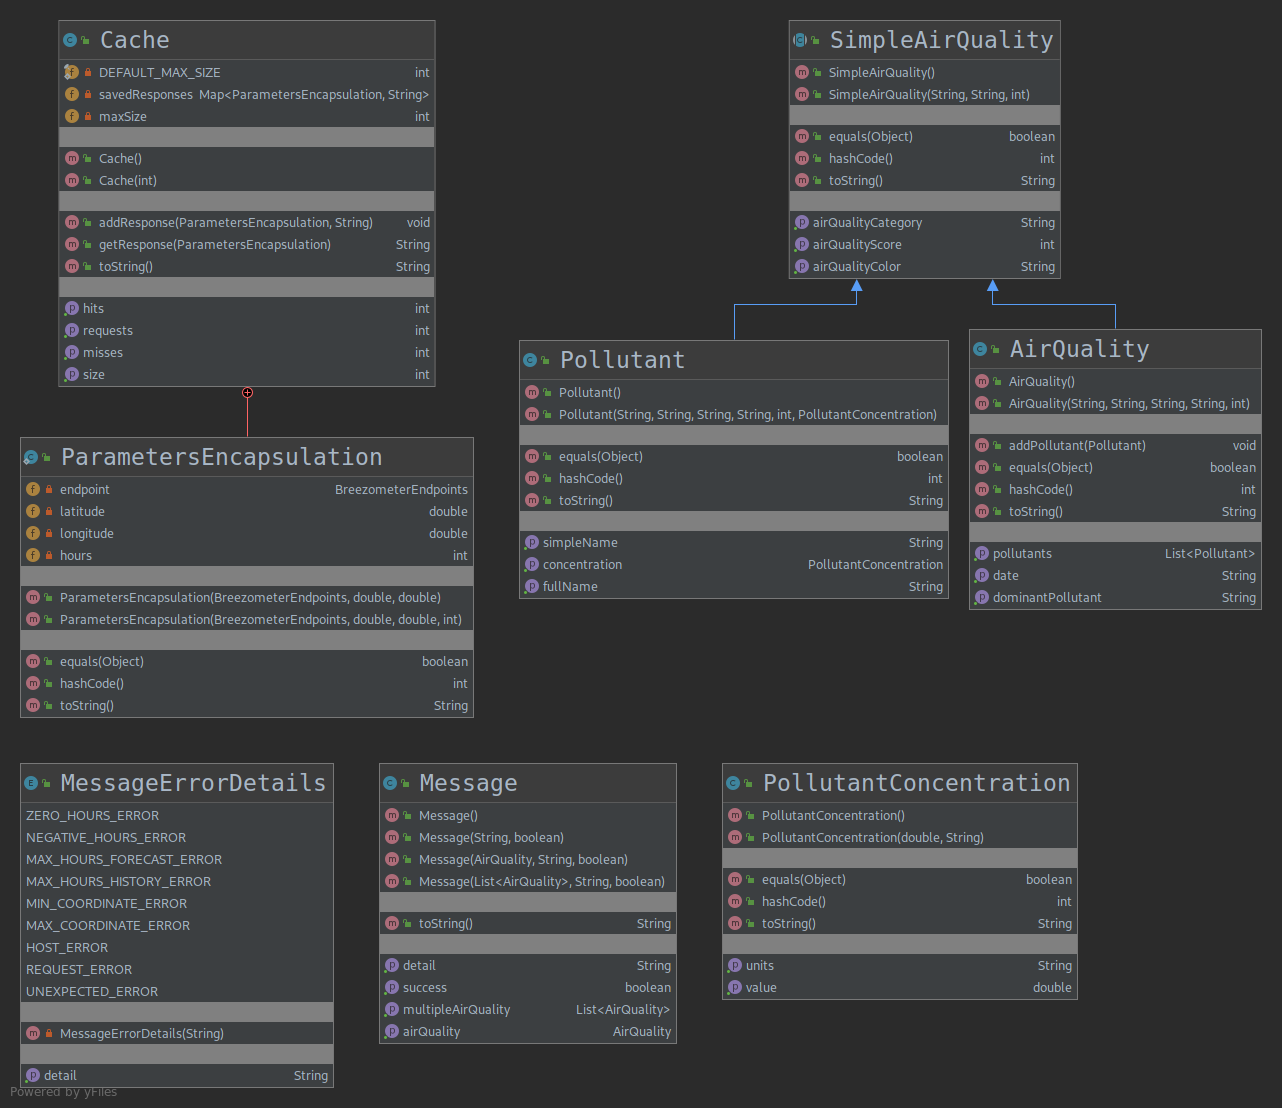
\includegraphics[width=0.90\textwidth]{images/model_diagram}
   \caption{Diagrama das classes do \textit{package \textbf{model}}.}
   \label{fig:model_diagram}
\end{figure}


\subsection{Package serializers}
De forma a poder fazer a "tradução" entre os dados recebidos do serviço externo e algumas das classes do \textit{model}, foram criados alguns \textit{deserializers} para esse efeito, como é possível verificar no diagrama da figura \ref{fig:serializers_diagram}. Para isso, foi usada a livraria \textit{Jackson}.
\begin{figure}[h]
   \centering
   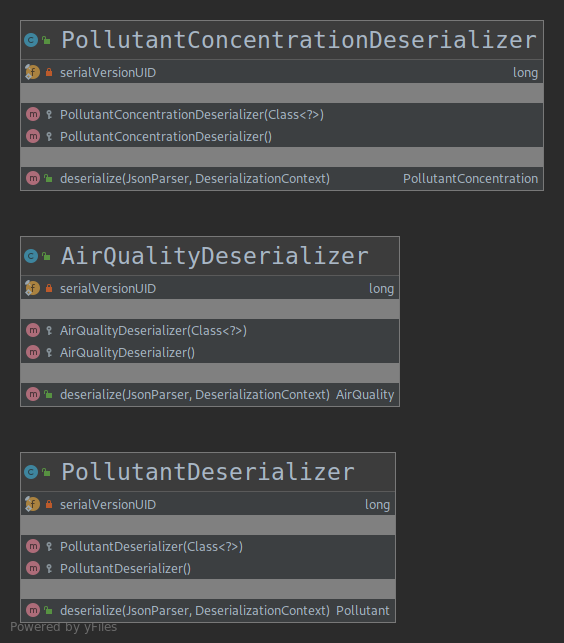
\includegraphics[width=0.90\textwidth]{images/serializers_diagram}
   \caption{Diagrama das classes do \textit{package \textbf{serializers}}.}
   \label{fig:serializers_diagram}
\end{figure}


\subsection{Package service}
De maneira a obter os dados necessários sobre a qualidade do ar, foi necessário criar um elo de ligação entre o \textit{back-end} criado e o serviço externo usado (\textit{BreezoMeter}), pelo que neste \textit{package} se encontram as classes que o permitem fazer. Quando a \textit{API} recebe um determinado pedido (excluindo o das estatísticas da cache), o método da classe \textbf{\textit{ConditionsController}} responsável por tratar do pedido "chama" o método \textit{requestApi} da classe \textbf{\textit{ConditionsController}} deste \textit{package} com o respetivo pedido, sendo que esta ultima faz um pedido ao serviço externo usando a classe \textbf{\textit{HttpBasic}} (disponibilizada pelo professor da disciplina numa das aulas práticas). A resposta do serviço externo é de seguida processada pelos \textit{deserializers} já descritos anteriormente e o objeto ou lista de objetos da classe \textbf{\textit{AirQuality}} são retornados ao método do \textit{controller} que tinha feito o pedido, encapsulados sob a forma dum objeto da classe \textbf{\textit{Message}}. Na figura \ref{fig:service_diagram} é possível encontrar a estrutura interna das classes deste \textit{package}.

\begin{figure}[h]
   \centering
   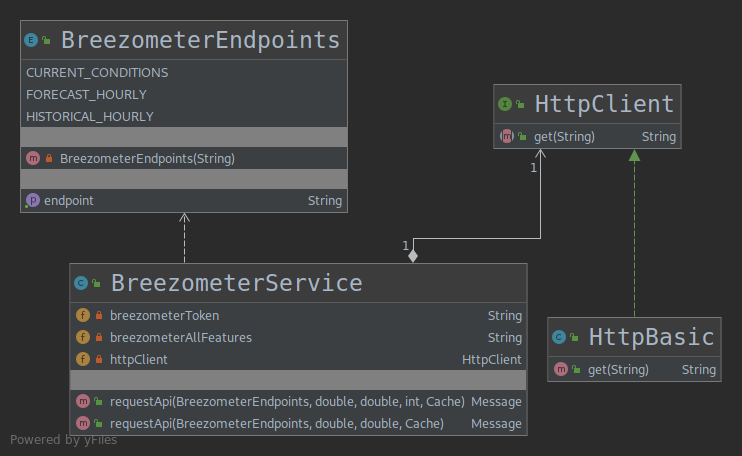
\includegraphics[width=0.90\textwidth]{images/service_diagram}
   \caption{Diagrama das classes do \textit{package \textbf{service}}.}
   \label{fig:service_diagram}
\end{figure}

% !TEX root = ../main.tex

\chapter{Garantia de qualidade}

\section{Estratégia geral usada para os testes}
Duma forma geral, a estratégia usada para fazer os testes foi usar \textit{TDD}, \textit{Test Driven Development}, e \textit{TLD}, \textit{Test Last Development}. Foi dado um especial destaque ao uso da primeira, como tentativa de mudar o hábito de fazer testes só depois de fazer todo o código, e aprender uma técnica de desenvolvimento de código aconselhada e que permite criar código fácilmente mantido. Contudo, foi impossível mudar completamente, e num só projeto, este \textit{mindset}. A ultima, apesar de não tão recomendada como a primeira, permite fazer código mais rápidamente e mais simples, numa primeira fase, mas alterações futuras são mais difíceis de serem feitas.

Quando usado \textit{TDD}, usualmente a classe sob a qual era pretendido serem feitos testes unitários foi criada primeiro, com toda a estrutura suposta e, posteriormente, foram criados os respetivos testes. Quando completada a criação destes, todo o código da respetiva classe era analisado, de forma a criar as \textit{features} supostas para que os testes passassem.

Para código mais complexo, foi usado \textit{TLD}, já que seria extremamente difícil de criar testes para algo que não se sabia inicialmente o comportamento. Muitas vezes, o código inicial deste tipo de classes foi feito mais como protótipo, de seguida criados testes para o comportamento que era esperado quando tudo funciona-se devidamente e por ultimo, melhorado o código desses protótipos de forma a criar classes com um comportamento adequado para o produto final.

É de sublinhar que não foi usada nenhuma abordagem \textit{BDD}.

Quanto a ferramentas usadas, para além do \textit{JUnit}, foi usado \textit{Mockito}, de forma a simular o comportamento de certos integrantes, e \textit{MockMvc} do \textit{Spring Boot}, de forma a simular os pedidos à \textit{API} criada e a obter as respetivas respostas.


\section{Testes unitários e de integração}
Numa primeira fase, foram criados testes unitários para cada os modelos principais e para os \textit{deserializers}. Posteriormente, foram feitos testes de integração quer ao serviço responsável por fazer a ligação ao serviço externo, quer ao controlador. Nas subsecções seguintes é explicado, duma forma geral, os testes feitos de cada tipo.

\subsection{Testes unitários}
\subsubsection{Modelos}
Quanto aos modelos, foram criados testes unitários para as classes \textbf{\textit{AirQuality}}, \textbf{\textit{Cache}}, \textbf{\textit{Pollutant}} e \textbf{\textit{PollutantConcentration}}, já que são os modelos que estão na base do negócio. Não foram criados testes para os restantes pelo simples motivo de que não apresentavam nenhum comportamento de risco, isto é, não têm nenhuma especificação que possa provocar erros no projeto, já que são apenas \textit{wrappers}, um das possíveis mensagens de erro e outro duma mensagem em si. 
Para as classes, foram feitos testes sobre o comportamento do método \textit{equals}, já que este foi modificado em todas as classes e em algumas, foi alterado o código auto-gerado pelo \textit{IDE}. Claro que noutras o código gerado pelo \textit{IDE} não foi alterado, mas poderia ser no futuro dado a utilização que foi dada a estas classes, pelo que se decidiu que era o melhor a ser feito de forma a controlar possíveis problemas.
Para além disso, sendo que a classe \textbf{\textit{AirQuality}} possuía um método que permitia adicionar novos poluentes em momentos distintos, isto é, não se tratava dum simples \textit{addPollutants}, onde seria dada a lista de poluentes toda, foram também feitos testes de forma a controlar o comportamento da adição de novos poluentes ou da não adição dos mesmos (exemplo dum destes testes na figura \ref{fig:air_pollutant_test}, onde é verificada se a ordem com que cada poluente é adicionado à qualidade do ar não afeta que duas qualidades do ar sejam diferentes).


\begin{figure}[h]
   \centering
   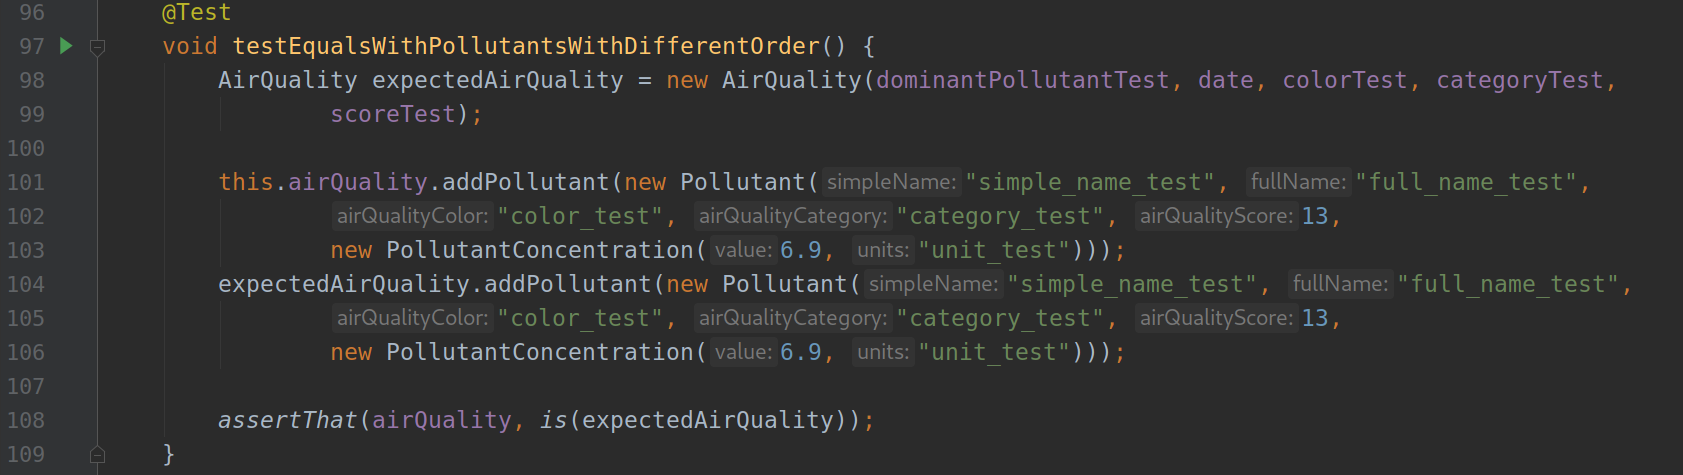
\includegraphics[width=0.90\textwidth]{images/air_pollutant_test}
   \caption{Exemplo dum código de teste da adição de poluentes a um objeto da classe \textbf{\textit{AirQuality}}.}
   \label{fig:air_pollutant_test}
\end{figure}

Já para a classe \textbf{\textit{Cache}}, sendo que esta apresentava um comportamento muito distinto das outras, foram criados testes diferentes. Principalmente testes que verificaram o tamanho da cache após excedido o tamanho máximo desta (exemplo do código em \ref{fig:cache_max}\footnote{no inicio de cada teste da cache são adicionados dois novos elementos, pelo que, ao todo, foram adicionados 4 elementos}), testes das condições iniciais e testes dos valores de cada uma das métricas de estatística.

\begin{figure}[h]
   \centering
   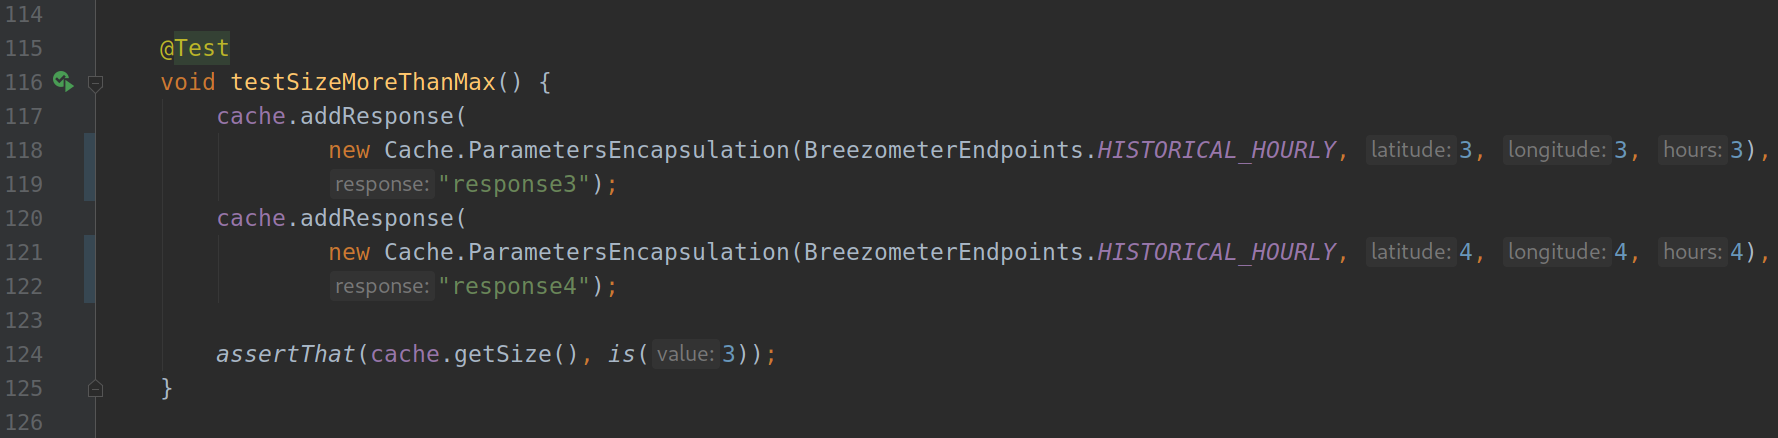
\includegraphics[width=0.90\textwidth]{images/cache_max}
   \caption{Exemplo do código de teste do tamanho máximo da cache.}
   \label{fig:cache_max}
\end{figure}


\subsubsection{Deserializers}
Sendo que foi alterado o comportamento original dos deserializers usados pelo \textit{Spring Boot}, as classes onde essa alteração foi feita tiveram de ser testadas. Desta forma, criaram-se testes unitários para as classes \textbf{\textit{AirQualityDeserializer}}, \textbf{\textit{PollutantDeserializer}} e \textbf{\textit{PollutantConcentrationDeserializer}}. 
Para testar o comportamento de cada uma destas, foi feito um teste similar em cada uma, em que foi dado uma \textit{string json} no mesmo formato das respostas obtidas nos \textit{requests} ao serviço externo e verificou-se se o objeto da respetiva classe criado era o suposto dado os parâmetros da \textit{string json}. 
Um exemplo dum destes testes pode ser encontrado na figura \ref{fig:serializer_test}, onde é criada uma \textit{string} com a formatação da concentração dum poluente que usualmente é recebida do serviço externo, sendo posteriormente esta "fornecida" aod respetivo \textit{deserializer} e por fim é verificado se o objeto retornado por este é o suposto.

\begin{figure}[h]
   \centering
   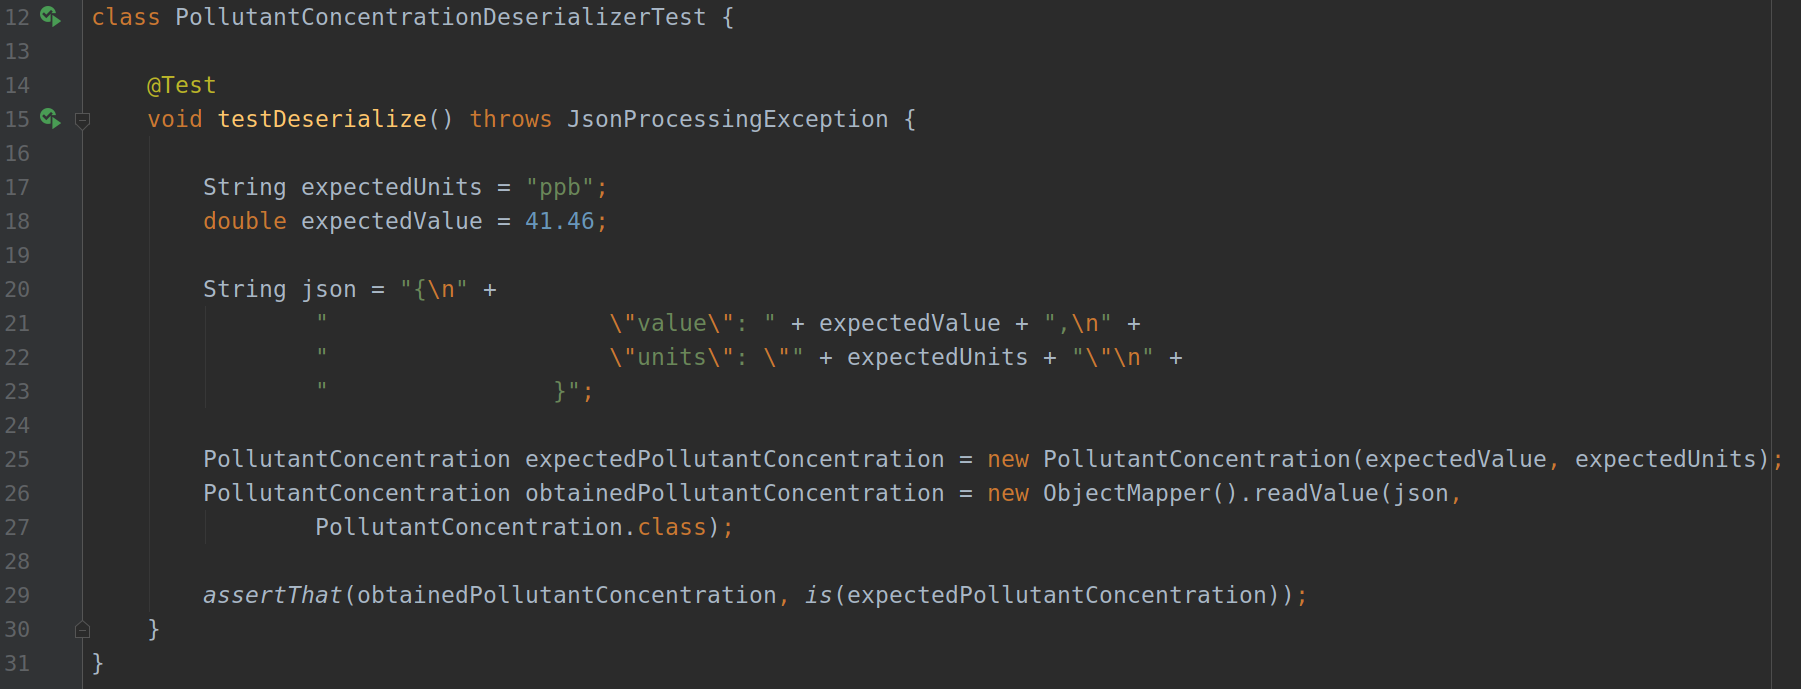
\includegraphics[width=0.90\textwidth]{images/serializer_test}
   \caption{Exemplo do código de teste do deserializer \textbf{\textit{PollutantConcentrationDeserializer}}.}
   \label{fig:serializer_test}
\end{figure}


\subsection{Testes de integração}
\subsubsection{Serviço}
Sendo que a classe \textbf{\textit{BreezometerService}} se liga a serviços externos e usa uma grande quantidade de componentes criados, foi necessário fazer alguns testes de integração para verificar se todas as partes funcionavam devidamente em conjunto. Para isso, foi dado uso ao \textit{MockBean} do \textit{Spring Boot}, de forma a simular o comportamento da interface \textbf{\textit{HttpClient}} e para, desta maneira, emular os resultados obtidos quando são feitos pedidos ao serviço externo. Um exemplo da configuração duma destas representações é demonstrada na imagem da figura \ref{fig:mock_http_client}, onde é obtida uma \textit{string json} com os parâmetros pretendidos através da utilização do método \textit{jsonAirQualityOnePollutantData} da classe \textbf{\textit{JsonSamples}} e se indica que, quando é feito um pedido ao à \textit{API} do \textit{BreezoMeter} dos dados da qualidade do ar atuais, para a latitude 10 e longitude 20, esta string deve ser retornada.

\begin{figure}[h]
   \centering
   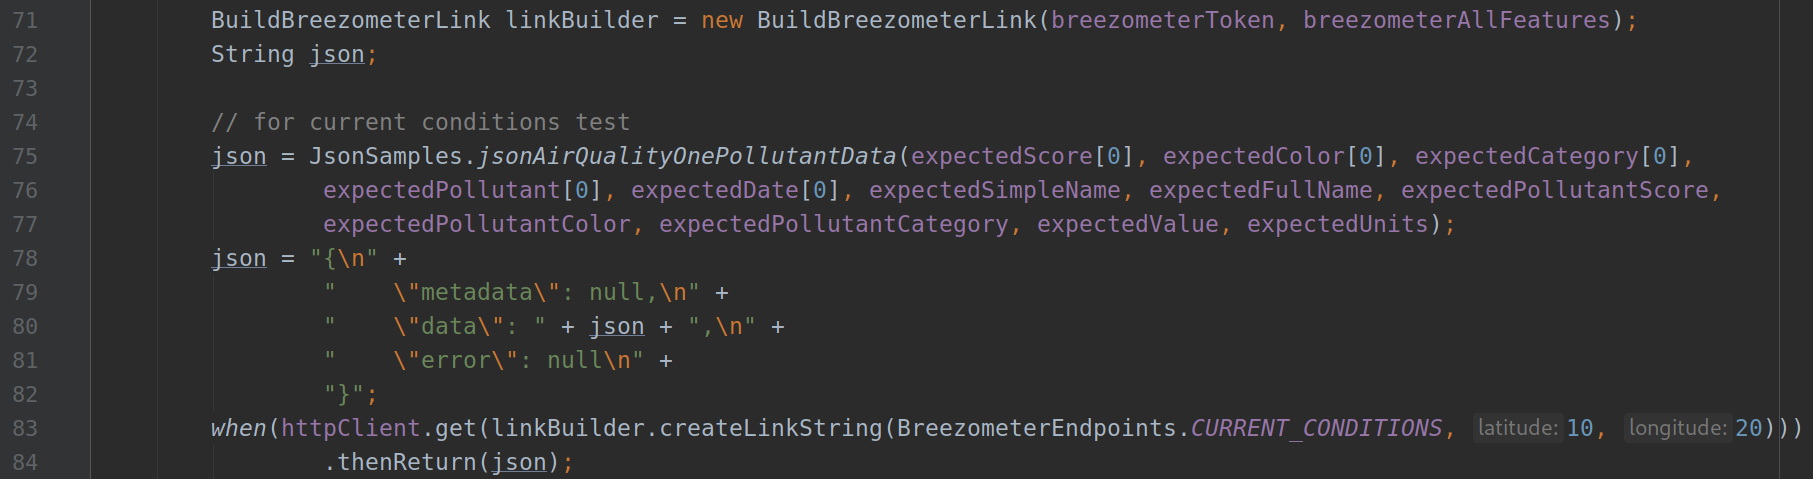
\includegraphics[width=0.90\textwidth]{images/mock_http_client}
   \caption{Exemplo duma simulação feita sob a interface \textbf{\textit{HttpClient}}, de forma a que esta dê uma dada resposta quando for feito um pedido especifico.}
   \label{fig:mock_http_client}
\end{figure}

Os testes desta classe passaram essencialmente por testar se quando feito um dado pedido, foi retornado o objeto da classe \textbf{\textit{Message}} suposto. Um exemplo dum destes testes pode ser consultado na imagem da figura \ref{fig:test_service}, onde é feito um pedido ao serviço \textbf{\textit{BreezometerService}} e é verificado se este retorna a mensagem suposta.

\begin{figure}[h]
   \centering
   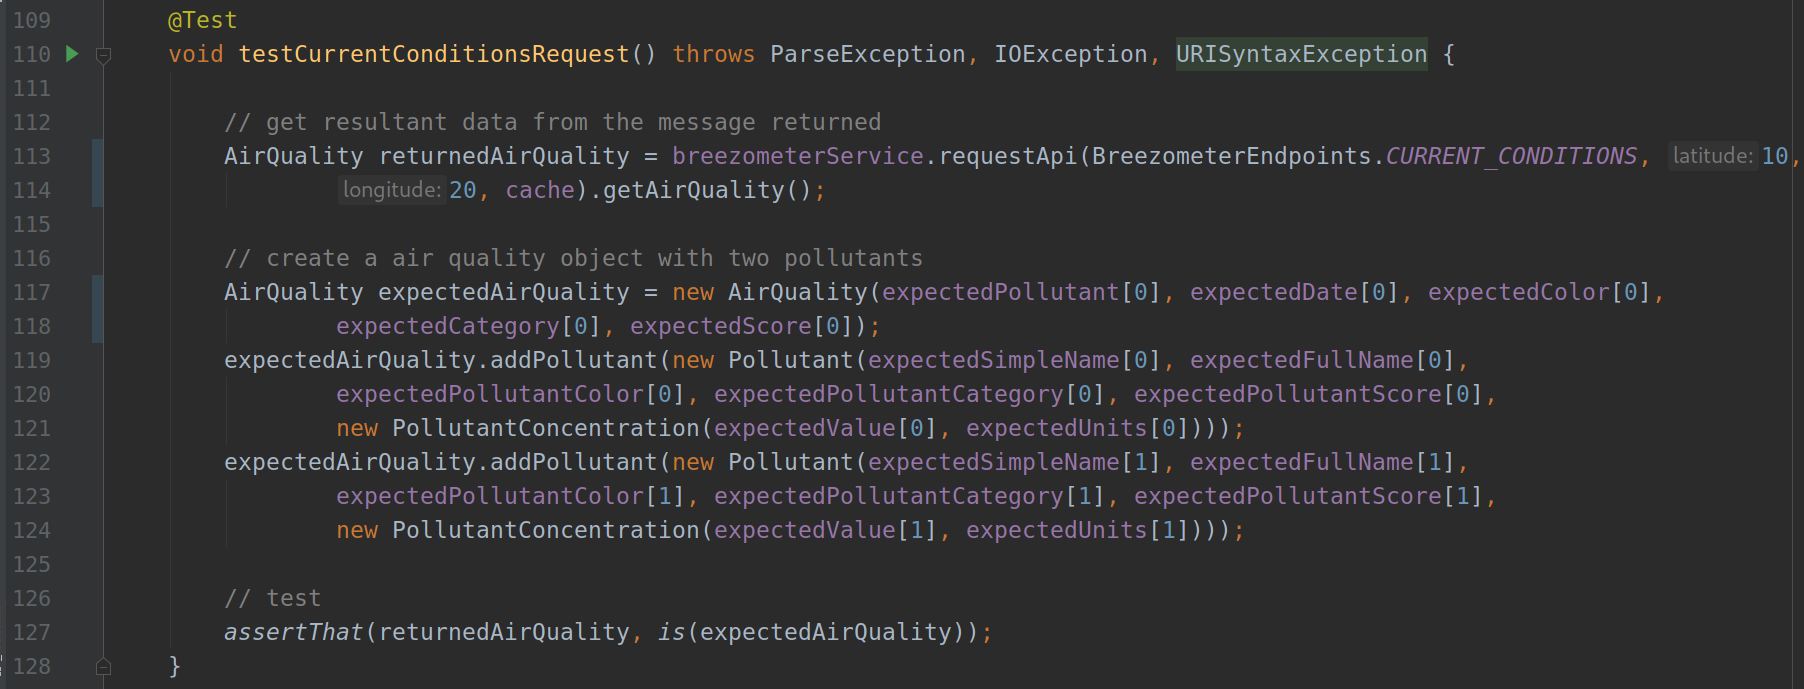
\includegraphics[width=0.90\textwidth]{images/test_service}
   \caption{Exemplo dum teste para verificação se quando feito um dado pedido ao serviço externo, o \textbf{\textit{BreezometerService}} retorna o pretendido.}
   \label{fig:test_service}
\end{figure}


\subsubsection{Controlador}
Pelo facto de na classe \textbf{\textit{ConditionsController}} se encontrarem todos os \textit{endpoints} e as especificações dos trabalhos a serem feitos quando é recebido um dado pedido na \textit{API}, foi necessário fazer uma grande quantidade de testes de integração sob esta classe, já que é ela que desencadeia a utilização de todas as outras classes criadas no projeto. Mais uma vez, foi usada a anotação \textit{MockBean} para permitir simular o comportamento da interface \textbf{\textit{HttpClient}}.

Posto isto, foram feitos testes não só para verificar se os vários métodos desta classe retornavam a mensagem da classe \textbf{\textit{Message}} devida, como também foram testadas as respostas dadas em \textit{json}, para confirmar que os resultados produzidos tinham a formatação esperada. Foram também induzidos erros quer nas respostas dadas pelo serviço externo, quer erros de execução inesperados, para confirmar se a \textit{API} tinha a capacidade de retornar as devidas mensagens de erro ou sucesso.

Para além de testes mais voltados para a interação com o serviço externo, foi também testado o serviço de cache usado, de forma a confirmar que quando feito um determinado conjunto de \textit{requests} à \textit{API}, os valores devolvidos quando pedidas as estatísticas da cache batiam certo.

Na figura \ref{fig:controller_test} é demonstrado um dos testes feitos, neste caso para confirmação de que o \textit{json} retornado quando feito um pedido das condições atuais possuía os valores e parâmetros corretos.

\begin{figure}[t]
   \centering
   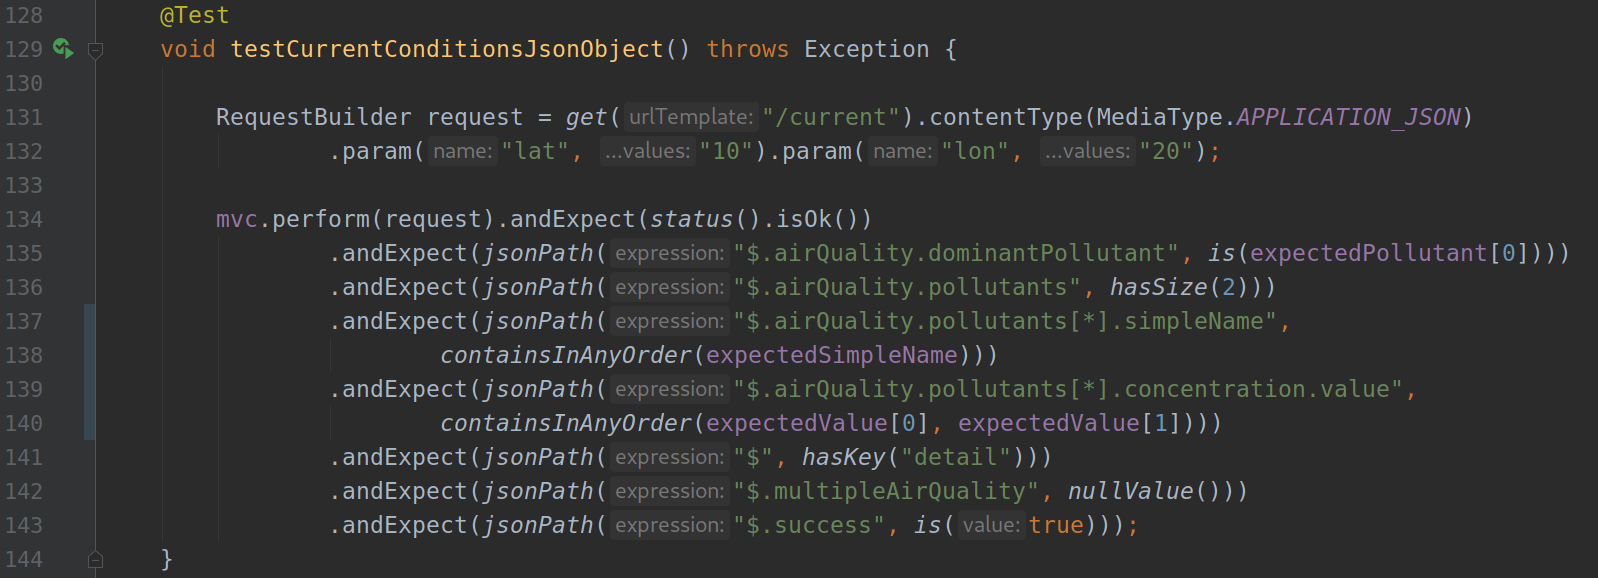
\includegraphics[width=0.90\textwidth]{images/controller_test}
   \caption{Exemplo dum teste feito à classe \textbf{\textit{ConditionsController}}, de forma a verificar se a resposta \textit{json} era a esperada para o pedido feito.}
   \label{fig:controller_test}
\end{figure}


\section{Testes funcionais}
De modo a criar os testes funcionais da interface criada, foi usada a ferramenta aconselhada durante as aulas da disciplina: \textit{Selenium IDE}. Através desta, é possível fazer facilmente a gravação das ações feitas numa determinada página a ser testada e exportar os resultados sob a forma duma classe de testes em \textit{JUnit}. Na figura \ref{fig:selenium_ide}, está um exemplo dum teste simples criado usando esta interface.

\begin{figure}[h]
   \centering
   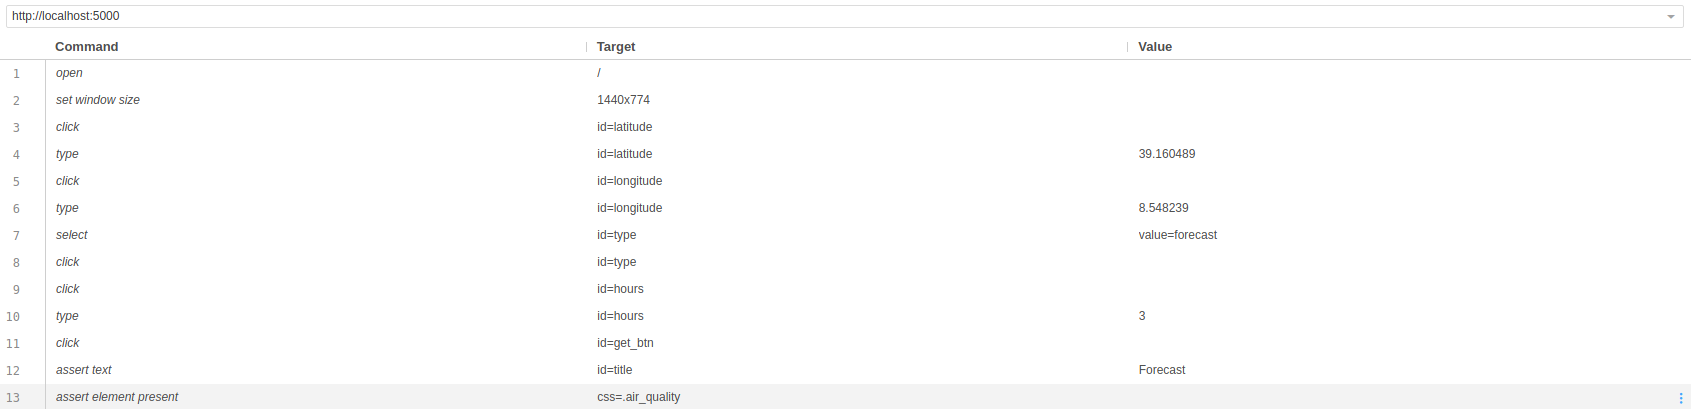
\includegraphics[width=0.90\textwidth]{images/selenium_ide}
   \caption{Exemplo dum teste criado no \textit{Selenium IDE}.}
   \label{fig:selenium_ide}
\end{figure}

Quanto aos testes criados, foi criado um novo projeto em \textit{Maven}, onde foram criados cada um dos testes. Estes encontram-se divididos por 3 classes: 
\begin{itemize}
   \item \textbf{\textit{ChooseTypeTests}}: testes para verificar se quando escolhido um tipo de pedido que não o \textit{current}, aparecia o \textit{input} \textit{hours} e desaparecia quando escolhido de novo o tipo \textit{current}, já que é só necessário especificar o número de horas para esses pedidos.
   \item \textbf{\textit{MessagesTests}}: testes para verificar se quando feito um pedido com sucesso,aparecia uma mensagem de sucesso numa caixa verde e quando feito um pedido incorreto, aparecia uma mensagem de erro numa caixa vermelha, sendo que as duas nunca poderiam aparecer em conjunto.
   \item \textbf{\textit{GetDataTests}}: testes para verificar se quando feito um pedido com sucesso dum determinado tipo, o titulo e o número de resultados obtidos era o correto.
\end{itemize}

Apesar do \textit{Selenium IDE} exportar o código dos testes, todo este código foi reformulado de forma a funcionar com \textit{JUnit 5}. Também foi feito algum refactor de forma a possuir só 3 classes separadas pelo tipo de testes e de maneira a evitar algumas repetições desnecessárias de código. Para testes onde foi necessário verificar se havia um determinado número específico de elementos na página, foi também necessário alterar o código obtido, já que aparentemente o \textit{Selenium IDE} só permite confirmar se um elemento está presente ou não na página e não o número de vezes que está.


\section{Análise de código estático}
Tal como pedido no guião do trabalho, era recomendada a utilização duma ferramenta de análise da qualidade do código. A que foi usada neste caso foi o \textit{Sonar Qube}, já que permite análise local de código (o repositório, até à data limite de entrega, foi privado) e pareceu bastante completa ao autor.

Esta ferramenta foi usada logo desde os estágios iniciais do projeto, de forma a evitar chegar a um estado avançado com uma grande quantidade de \textit{bugs} ou \textit{code smells}. Sendo assim, desde o inicio, qualquer nova versão do código da \textit{API} foi verificado no \textit{Sonar Qube}, de maneira não haverem quaisquer tipos de \textit{bugs} e \textit{code smells}, pelo que caso algum aparecesse em código feito recentemente, ser imediatamente corrigido.

Apesar de não ter tido uma grande quantidade deste tipo de problemas, houve um que se destacou pela sua persistência no inicio: criação de variáveis e métodos em \textit{Snake case} e não \textit{CamelCase}. Isto deve-se principalmente ao facto do autor usar \textit{python} como linguagem de programação de referência no dia a dia e não estar completamente habituado a usar \textit{java}. Ainda que este tipo de problemas fosse classificado como \textit{Minor}, é algo importante a ser usado quando se programa nesta linguagem, já que é o \textit{standard} e acaba por tornar o código de fácil leitura a programadores que não o autor inicial.

Também foi usada esta ferramenta, em conjunto com o \textit{JaCoCo}, de maneira a obter uma análise da cobertura dos testes criados. Desde o inicio que foi usado um \textit{Quality Gate} igual ao usado por default, mas com um mínimo de cobertura de código de 70\%, já que para desenvolvimento parece ser suficiente. Aquando da conclusão da \textit{API}, foi obtida uma cobertura de 90.3\%, o que parece ser ótimo.

Na imagem da figura \ref{fig:sonar} é possivel encontrar um \textit{print} da \textit{dashboard} deste projeto no 
\textit{Sonar Qube}, onde se pode confirmar que foram reduzidos a zero o número de \textit{bugs}, vulnerabilidades, \textit{Security Hotspots} e de \textit{Code Smells}, bem como a percentagem de \textit{Coverage} é superior a 90\%. Já na figura \ref{fig:sonar_activity}, é possível confirmar que a quantidade de problemas no código manteve-se sempre baixa, sendo que no inicio foram o mais rápidamente eliminados os erros existentes.

\begin{figure}[h]
   \centering
   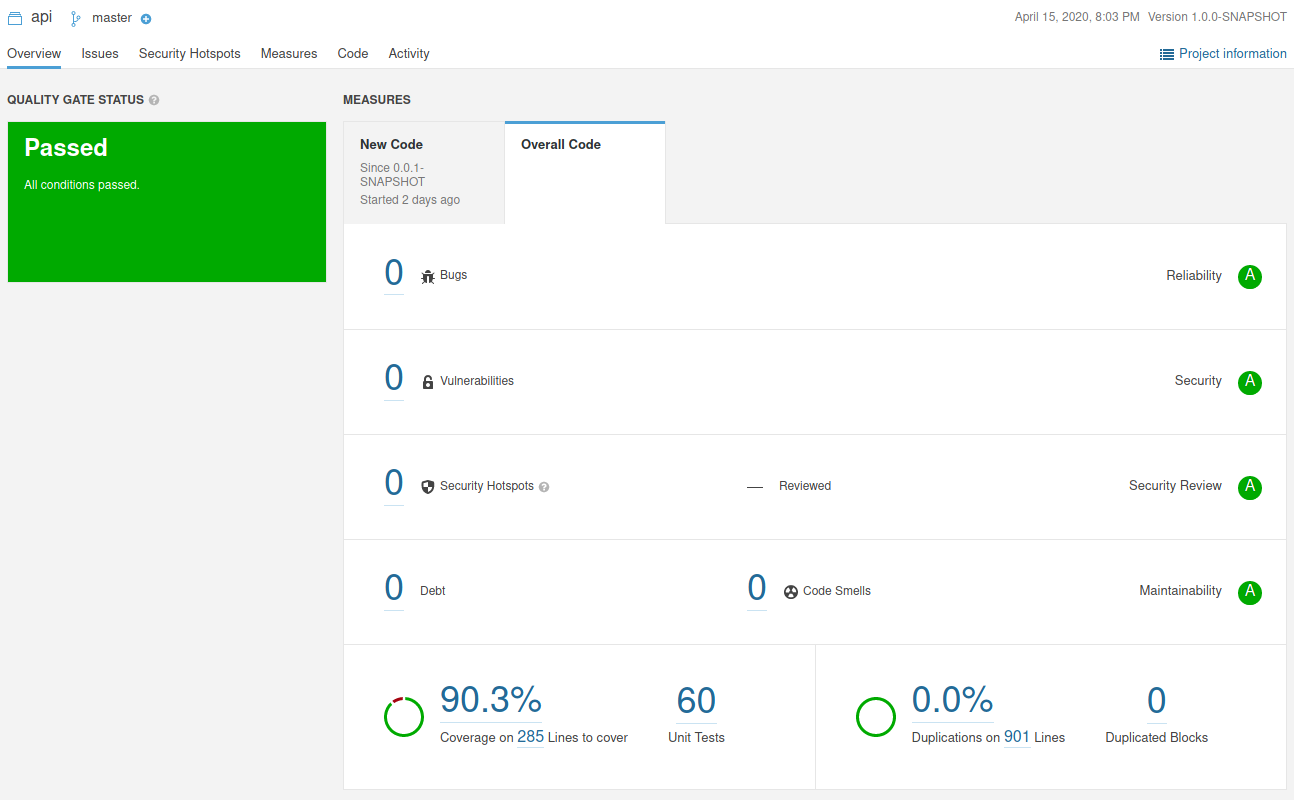
\includegraphics[width=0.90\textwidth]{images/sonar}
   \caption{\textit{Dashboard} do projeto no \textit{SonarQube}.}
   \label{fig:sonar}
\end{figure}

\begin{figure}[h]
   \centering
   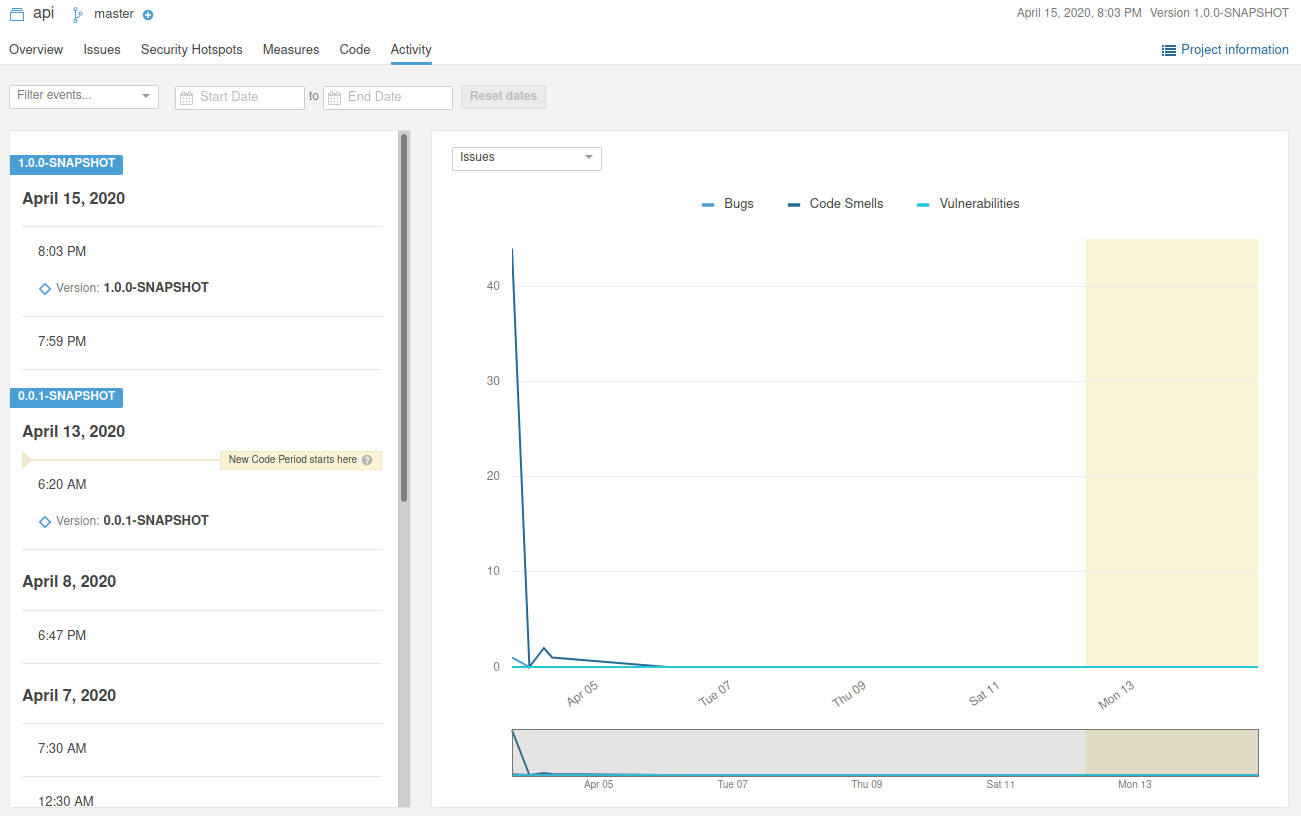
\includegraphics[width=0.90\textwidth]{images/sonar_activity}
   \caption{Evolução dos problemas do código da \textit{API} ao longo do desenvolvimento.}
   \label{fig:sonar_activity}
\end{figure}


\end{document}
